\chapter{Selección y Estudio de los conjuntos de datos}

En el anterior capítulo, hemos revisado el estado actual de los encodings en los modelos de series temporales, y hemos realizado cinco propuestas teniendo como principal concepto el uso de ventana para aumentar el contexto explícito de los datos, y la hibridación de diferentes métodos vistos mediante el uso de encodings ponderados. Pero con la formulación no es suficiente, ya que debemos comprobar su efectividad de manera empírica, realizando para ello diversos experimentos sobre diferentes conjuntos de datos.\\

Por tanto, en este apartado, introduciremos los diferentes conjuntos de datos seleccionados, analizando su contexto de extracción y algunas características básicas. Debido a su extenso tamaño, resulta complejo y costoso realizar representaciones gráficas sobre los datos, por lo que sólo se realizarán cuando sea posible por su extensión.

\section{Electricity Transformer Dataset (ETT)}

Este conjunto de datos fue empleado en la publicación original de Informer~\cite{zhou2021informerefficienttransformerlong}, y a raíz de su utilización, multitud de modelos posteriores han hecho uso de este dataset, a modo de conjunto de referencia para la comparativa entre arquitecturas y sus variantes. Contiene información acerca de dos transformadores eléctricos, que se encuentran en diferentes subestaciones, y se recogen datos acerca de su carga y la temperatura del aceite en el cual se encuentran sumergidos los componentes para mejorar el aislamiento.\\

Como ya mencionamos en la introducción, disponer de una buena estimación de la carga eléctrica necesaria para abastecer a una región y controlar la salud de los diferentes componentes del sistema para evitar caídas es clave para el aprovechamiento de recursos. Pero las condiciones y necesidades en cada instante pueden ser diferentes; la demanda puede verse afectada por el día de la semana, la existencia de vacaciones, estaciones del año, climatología, temperaturas... Todas ellas afectan de manera directa a las necesidades y a la eficiencia del sistema, por lo que la complejidad del problema hace que en muchas ocasiones las decisiones se tomen teniendo al alza, sobreproduciendo y sobredimensionando las necesidades para evitar problemas de abastecimiento. Sin embargo, esto no es eficiente, ya que se están desaprovechando recursos tanto en la producción de energía, en caso de usar fuentes no renovables, y en la producción e instalación de equipos.\\

Si conseguimos buenos resultados de predicción, podríamos idealmente reducir los recursos pero mantener un sistema estable. Y una componente clave de este ecuación es supervisar el estado del sistema, y en este dataset, concretamente, de los transformadores. La variable temperatura de aceite, que a priori parecía no demasiado útil, es clave en este conjunto de datos para detectar posibles anomalías que puedieran provocar un mal funcionamiento o problemas de suministro de manera bastante directa, ya que las temperaturas extremas afectan negativamente a su rendimiento. Bajo esta justificación, los autores extrajeron el conjunto de datos proveniendo de dos transformadores, y que recogen 2 años de datos minuto a minutogracias a una plataforma de recolección realizada con la colaboración de \textit{Beijing Guowang Fuda Science \& Technology Development Company}.\\

Originalmente, fueron extraídas más series de más transformadores, pero sólo se hicieron públicos dos, agrupados en la variante ETT-Small, que podemos encontrar en su correspondiente repositorio de GitHub~\cite{zhou2021etdataset}. Los datos provienen de dos regiones de una provincia de China, denominadas ETT-small-m1 y ETT-small-m2. En total, los dos años se traduce 70.080 puntos de datos por cada transformador. Adicionalmente, podemos encontrar dos variantes preprocesadas para realizar el forecasting hora a hora, reduciendo así el esfuerzo de cómputo necesario. Siguiendo la misma estructura de notación que los anteriores, reciben los nombres ETT-small-h1 y ETT-small-h2, siendo la h el indicativo de ``horario''.\\

Cada instante de los datos consta de 8 características, incluyendo el timestamp y 7 variables diferentes, entre la que se encuentra la temperatura del aceite:

\begin{itemize}
	\item \textbf{date}: Fecha y hora exacta en la que se realizó la medición, permitiendo situar cada registro en la secuencia temporal.
	
	\item \textbf{HUFL} (\textit{High Useful Load}): Componente útil de la carga cuando el transformador trabaja a un nivel alto de demanda. Representa la parte de la energía efectivamente utilizada para alimentar la red.
	
	\item \textbf{HULL} (\textit{High Useless Load}): Componente no útil de la carga en nivel alto, asociada principalmente a pérdidas y consumos del propio sistema del transformador cuando está sometido a alta demanda.
	
	\item \textbf{MUFL} (\textit{Middle Useful Load}): Componente útil de la carga cuando el transformador opera a un nivel medio de demanda, asociado a un funcionamiento más estable y eficiente que en carga alta.
	
	\item \textbf{MULL} (\textit{Middle Useless Load}): Componente no útil de la carga en nivel medio, de nuevo, vinculada a pérdida y consumo propio del sistema.
	
	\item \textbf{LUFL} (\textit{Low Useful Load}): Componente útil en baja carga, es decir, en baja demanda energética.
	
	\item \textbf{LULL} (\textit{Low Useless Load}): Componente no útil de la carga en nivel bajo. En este caso, es posible que las pérdidas puedan ser más significativas en proporción a la potencia de salida.
	
	\item \textbf{OT} (\textit{Oil Temperature}): Temperatura del aceite del transformador, marcada por los autores del conjunto de datos como posible variable a estimar en caso de tratar los datos como un problema de predicción de única variable objetivo. Como ya comentábamos, se trata de una componente clave, ya que el sobrecalentamiento puede reducir su vida útil y provocar fallos, mientras que una temperatura demasiado baja puede empeorar la viscosidad del aceite y sus capacidades.
\end{itemize}

El interés de escoger este dataset reside en la extensión relativamente reducida del mismo, ya que buena parte de los conjuntos de datos de gran tamaño suelen alcanzar los millones de instancias, y resulta complicado realizar ajuste de parámetros si los tiempos de ejecución superan las varias semanas. Además, supone un buen conjunto para evaluar los métodos de encoding propuestos en horizontes de tamaño medio.\\

Como podríamos intuir, y además, así nos remarcan sus autores~\cite{zhou2021etdataset}, este conjunto de datos presenta características típicas de series temporales reales. En primer lugar, se observan patrones estacionales, tanto a nivel diario (por ejemplo, horas cercana al almuerzo y la cena son mayores), semanal (debido a los fines de semana) e incluso a nivel de estación del año o mensual, pasando por los días festivos; también se aprecian tendencias a medio y largo plazo, afectando al nivel medio de producción y posiblemente asociado a factores como el crecimiento de la demanda energética en general.Y podemos encontrar ruido, fruto de variaciones puntuales, errores de medición o condiciones imprevistas. Por tanto, nos permite analizar factores clave propios de un problema de predicción a largo plazo.\\

Toda esta información la podríamos apreciar si representamos gráficamente los datos, pero puede ser complicado debido a la extensión de la serie y su variabilidad, que podría hacer que se pisen los puntos entre sí. Pero sí que podemos analizar gráficamente su autocorrelación, ya que cada variable sigue un comportamiento lo suficientemente diferente y podemos apreciar si existe información estacional. 

\begin{figure}[!ht]
	\centering
	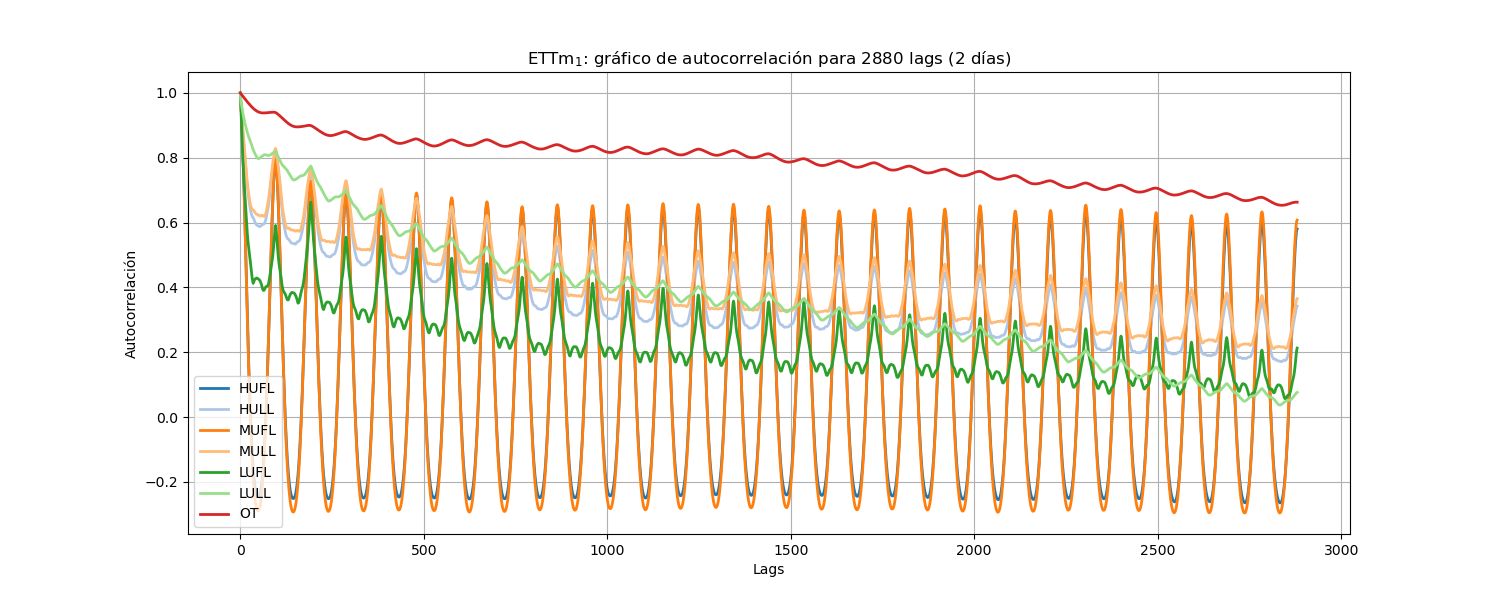
\includegraphics[scale=0.37]{img/etth1_autocorrelacion.png}
	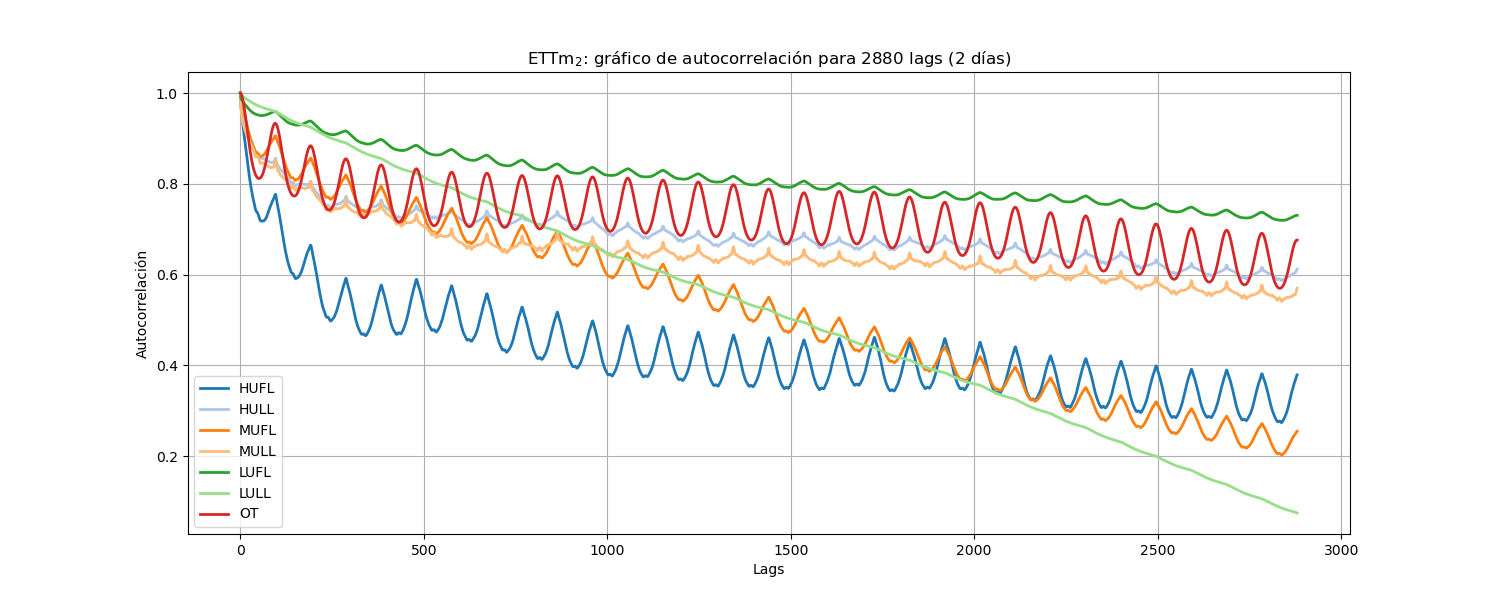
\includegraphics[scale=0.37]{img/etth2_autocorrelacion.png}
	\caption{ETT: gráficos de autocorrelación para ETTH$_1$ y ETTH$_2$}
	\label{autoett}
\end{figure}

En la figura \ref{autoett}, podemos apreciar el gráfico normalizado para las dos regiones, minuto a minuto, para una sucesión de 2880 lags, que equivale a una longitud de 2 días completos, para así observar información de estacionalidad a corto plazo.

\begin{itemize}
	\item Para el primer transformador, \textbf{ETTh1}, los valores parecen oscilar de manera considerable, pero muestran un comportamiento claramente estacional en todas sus variables. Si bien resulta complicado estimar el período concreto seguido, podemos ver claramente su evolución, y que no es una red estacionaria para ninguna de sus componentes. Por tanto, métodos clásicos como ARIMA no serían útiles, pero otros modelos más avanzados que sean capaces de recoger la semántica dada por cada estación nos permitiría obtener un buen rendimiento. A lo largo del tiempo, los valores de ACF prácticamente no varían, especialmente en carga media, cuyos valores ACF siempre oscilan en la misma amplitud y media. En cuanto a la correlación inmediata con el valor inmediatamente anterior, resulta ser bastante alta, por lo que podría ser una buena base para el modelado, pero sigue siendo necesario distinguir la estacionalidad para minimizar el error.
	\item En el caso de \textbf{ETTh2}, el comportamiento es algo diferente. Si bien la correlación con el anterior valor sigue siendo alta, y la estacionalidad se mantiene, la amplitud de los picos es bastante menor, indicando valores menos cambiantes y estables. Curiosamente, el comportamiento de \textit{LULL} contrasta bastante con el resto, ya que parece tener una tendencia claramente decreciente a cero. Sin embargo, para concocer la existencia de estacionalidad en dicha variable necesitaríamos ampliar demasiado el número de lags, y por tanto, dificultar el visualizado del resto de series. Basándonos en el otro transformador y las descripciones dadas de las variables, sí que se tratará de una serie también estacional, pero su período es de mayor amplitud y no apreciable.
\end{itemize}

En el caso de las variantes horarias, se trata simplemente de la misma información muestreada, por lo que el comportamiento será bastante similar al visto aquí pero con intervalos entre muestreos más largo (60 veces mayor exactamente).\\

De manera previa, a la vista de la información dada por los gráficos de autocorrelación, podemos intuir además de que el segundo conjunto puede ser más complejo de modelar, ya que además este no fue utilizado por el paper original de Informer ni buena parte de los modelos posteriores que se probaron. La mayoría optan por evaluar únicamente el primer transformador.
